\documentclass[a4paper,10pt]{article}

%A Few Useful Packages
\usepackage{marvosym}
\usepackage{fontspec} 					%for loading fonts
\usepackage{xunicode,xltxtra,url,parskip} 	%other packages for formatting
\usepackage{wrapfig}
\RequirePackage{color,graphicx}
\usepackage[usenames,dvipsnames]{xcolor}
\usepackage[big]{layaureo} 				%better formatting of the A4 page
% an alternative to Layaureo can be ** \usepackage{fullpage} **
\usepackage{supertabular} 				%for Grades
\usepackage{titlesec}					%custom \section
\usepackage{enumitem}

%Setup hyperref package, and colours for links
\usepackage{hyperref}
\definecolor{linkcolour}{rgb}{0,0.2,0.6}
\hypersetup{colorlinks,breaklinks,urlcolor=linkcolour, linkcolor=linkcolour}

%FONTS
\defaultfontfeatures{Mapping=tex-text}
%\setmainfont[SmallCapsFont = Alegreya SC]{Alegreya}
\setmainfont[SmallCapsFont = Alegreya]{Alegreya}

%CV Sections inspired by: 
%http://stefano.italians.nl/archives/26
\titleformat{\section}{\Large\scshape\raggedright}{}{0em}{}[\titlerule]
\titlespacing{\section}{0pt}{3pt}{3pt}
%Tweak a bit the top margin
%\addtolength{\voffset}{-1.3cm}

%Italian hyphenation for the word: ''corporations''
\hyphenation{im-pre-se}

%-------------WATERMARK TEST [**not part of a CV**]---------------
\usepackage[absolute]{textpos}

\setlength{\TPHorizModule}{30mm}
\setlength{\TPVertModule}{\TPHorizModule}
\textblockorigin{2mm}{0.65\paperheight}
\setlength{\parindent}{0pt}

%--------------------BEGIN DOCUMENT----------------------
\begin{document}

%WATERMARK TEST [**not part of a CV**]---------------
%\font\wm=''Baskerville:color=787878'' at 8pt
%\font\wmweb=''Baskerville:color=FF1493'' at 8pt
%{\wm 
%	\begin{textblock}{1}(0,0)
%		\rotatebox{-90}{\parbox{500mm}{
%			Typeset by Alessandro Plasmati with \XeTeX\  \today\ for 
%			{\wmweb \href{http://www.aleplasmati.comuv.com}{aleplasmati.comuv.com}}
%		}
%	}
%	\end{textblock}
%}

\pagestyle{empty} % non-numbered pages

\font\fb=''[cmr10]'' %for use with \LaTeX command

%--------------------TITLE-------------
\par{\centering
		{\small In the Name of Allah}\\
		\vspace{22mm}
		{\Huge Rouhollah \textsc{Farhang}
	}\bigskip\par}

%--------------------SECTIONS-----------------------------------
%Section: Personal Data
\section{Personal Data}

%\begin{wrapfigure}{r}{0.25\textwidth}
%\end{wrapfigure}

%\begin{minipage}[b]{0.75\textwidth}
\begin{tabular}{rl}
    \textsc{Place and Date of Birth:} & Isfahan, Iran | April 1983 \\
    \textsc{Address:}   & No 1, Nekoudeqqat alley, Jalali alley, Moallem st., Tehran\\
    \textsc{Phone:}     & +98 912 1774416\\
    \textsc{email:}     & \href{mailto:rouhollah.farhang@gmail.com}{rouhollah.farhang@gmail.com}\\
    \textsc{GitHub:}	& \href{https://github.com/rfar}{rfar@GitHub}
\end{tabular}
%\end{minipage}


%--------------------------------------------------
%Section: Work Experience at the top
\section{Work Experience}
\begin{tabular}{r|p{11cm}}
\emph{Current} &Project Manager and Full-stack Web Developer at Rastafann\\\textsc{Feb 2015}& \footnotesize{Currently managing, as well as partly developing, an online Islamic books library  with full-text search named \href{https://ablibrary.net}{ABLibrary} with offline versions available for Windows, iOS and Android.}\\\multicolumn{2}{c}{} \\
\textsc{Feb 2015} &Programmer at Fat'h Research Center\\\textsc{Jun 2013}& \footnotesize{Developed cross-platform desktop application using C++/Qt.}\\\multicolumn{2}{c}{} \\
\textsc{Feb 2014} & Network Programmer at \textsc{Web R\&D Center}\\\textsc{May 2013}& \footnotesize{Worked as a network programmer performing network traffic capture under linux.}\\\multicolumn{2}{c}{} \\
 \textsc{Nov 2013} & Design Engineer at \textsc{KavoshCom R\&D} \\\textsc{Sep 2009}&\footnotesize{Worked on improving GPS/GLONASS algorithms.}\\\multicolumn{2}{c}{} \\
\textsc{2007-2008} & Researcher at Acoustics Research Center, Tehran \\&\footnotesize{Extensive knowledge on Infrasound, Infrasonic Sensors, Data Centers and Interferometry.}\\\multicolumn{2}{c}{}
\end{tabular}

%--------------------------------------------------
%Section: Education
\section{Education}
\begin{tabular}{rl}	
 \textsc{Jan} 2009 & MSc in \textsc{Communications Engineering}, \textbf{Sharif University of Technology}, \\
& Tehran | Major: Electrical Engineering\\
& Thesis: ``Throughput Analysis of Routing Algorithms in 802.11s-Based Wireless \\
& Mesh Networks'' | \small Advisor: Dr Farid \textsc{Ashtiani}
\\&\\
\textsc{Sep} 2006 & BSc in \textsc{Electrical Engineering}, \normalsize\textbf{Iran University of Science and Technology}, \\
& \normalsize Tehran\\
& Thesis: ``Positioning by TOA Estimation in Wireless Multipath Channels''\\
& | \small Advisor: Dr MohammadHossein \textsc{Kahaie}
\end{tabular}

\textsc{Courses Attended}
\begin{itemize}[topsep=-3pt, itemsep=-3pt]
\item Digital Communications
\item Stochastic Processes
\item Data Networks
\item Coding Theory
\item Optimization Theory
\item Spread Spectrum Communication
\item Queuing Theory
\item DSP
\end{itemize}

%--------------------------------------------------
%Section: Scholarships and additional info
\section{Awards and Certificates}
\begin{tabular}{r|p{11cm}}%{rl}
\textsc{Feb} 2011 & \textsc{2\textsuperscript{nd} Rank in the 24\textsuperscript{th} Khwarizmi International Festival}\\
& \footnotesize{Was member of the team winning the award for designing, manufacturing and testing a space GPS receiver for positioning satellites in LEO.}\\\multicolumn{2}{c}{}\\
\textsc{May} 2006 & \textsc{CCNA: Cisco Certified Network Associate}\\
& \footnotesize{Graduated the course held under supervision of AsanWeb Sharif with excellent grade.}\\\multicolumn{2}{c}{}\\
\textsc{June} 2005 & \textsc{ZD: Zertifikat Deutsch als Fremdsprache}\\
& \footnotesize{Attended the course and passed the examination at Iran Language Institute (ILI)}.
%\setmainfont[SmallCapsFont=Fontin SmallCaps]{Fontin-Regular}: 730 (\textsc{q:50;v:39}) 96\textsuperscript{th} percentile; \textsc{awa}: 6.0/6.0 (89\textsuperscript{th} percentile)
\end{tabular}

%--------------------------------------------------
\section{Programming Skills}
\begin{tabular}{rl}
Having Basic Skills at:
					& Common Lisp (especially the SBCL implementation)\\
					& Racket Language\\
					& Rust Programming and its ownership system\\
					& Objective-C Programming\\
					& GNU Make\\
					& Android SDK Programming\\
					& Haskell Programming\\
					& OCaml Programming\\
					& Functional Type-Level Programming\\
					& Quantum Computing\\
					\\
Skilled at:
				& Functional Programming in Clojure\\
				& Relational Theory and PostgreSQL\\
				& Golang Server-side Programming\\
				& Emacs \& Emacs Lisp\\
				& C Programming\\
				& Python Programming\\
				& Swift 5 \& Cocoa Framework\\
				& Java Programming, including Java 8 features\\
				& Object-Oriented Programming\\
                & Parallel Programming using nVidia CUDA\\
				& MATLAB Programming\\
				& Software Design Patterns\\
				& Version Control using Git\\
				& Linux OS\\
				& Node.js\\
				& {\fb \LaTeX}\\%\setmainfont[SmallCapsFont=Fontin SmallCaps]{Fontin-Regular}\\
				\\
Proficient in: & C++ Programming (including modern C++)\\
				& Qt Application Framework\\
				& JavaScript (including ES6+) and numerous front-end libraries\\
				& \hspace{1cm} including Ramda, Lodash, Moment.js, PDF.js and Lovefield\\
				& React Framework and its ecosystem (e.g. Redux and react-router)\\
				& Webpack \& Babel

\end{tabular}

%--------------------------------------------------
\section{Other Skills}
\begin{tabular}{rl}
Cryptography:
	& PGP \& OpenPGP\\
	& Public-Key Cryptography\\
	\\
Reverse Engineering:
	& Familiar with detailed ELF binary structure\\
	& Static Binary Analysis\\
	& Dynamic Binary Analysis\\
	& IDA Pro 7 Disassembler\\
	& Radare2 Reverse Engineering Framework\\
	\\
Bitcoin \& Blockchain\\
	\\
Emacs:
	& Emacs Lisp language\\
	& Org Mode (an advanced outliner, task manager, etc.)\\
	& Magit (a textual interface to Git)\\
	& Cider (Clojure IDE)\\
	& SLY \& SLIME (Common Lisp and Scheme IDEs)\\
\end{tabular}

%--------------------------------------------------
\section{Software Skills}
VS Code (JavaScript/React and Golang), LightTable (Clojure IDE),
Qt Creator/Designer, Xcode, Eclipse, Tmux (terminal multiplexer), Zsh (bash alternative), iTerm (macOS terminal emulator), Android Studio, MS Visual Studio, Valgrind, JetBrains IntelliJ \& Pycharm, Oracle NetBeans, Sublime Text, SmartGit, SourceTree, Tower (macOS Git client), GitExtensions, Doxygen, Texmaker, Texpad (macOS {\fb \LaTeX} editor), KDiff, Beyond Compare, Wireshark

%--------------------------------------------------
%Section: Languages
\section{Languages}
\begin{tabular}{rl}
\textsc{Persian:} & Mothertongue\\
\textsc{English:} & Fluent\\
\textsc{French:} & have a good command of\\
\textsc{German:} & have a rather good command of\\
\textsc{Arabic:} & Intermediate Written Knowledge
\end{tabular}

%--------------------------------------------------
\section{Interests}
Functional Programming\\
Reverse Engineering

%--------------------------------------------------
\section{About Me}

\begin{wrapfigure}{r}{0.2\textwidth}
%\centering
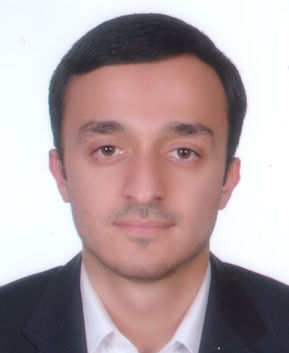
\includegraphics[scale=.25]{resources/me.jpg}
\end{wrapfigure}

Since as far back as school years I've had a tendency towards developing fresh skills and trying new things. However, having majored in Electrical Engineering and minored in Communications Engineering was not a perfect match for my insatiable desire for reading and learning---of which learning French and German languages has been an example.

On the other hand, with programming not only could I cruise along the road of learning every single day by learning new techniques, but also had the opportunity to design and develop in line with my tastes as it is, sort of, an art. Besides that, in the world of programming there is almost no gap between the new techniques that I learn and their real world usage.

I'm kind of a computer and technology geek---following the latest news, tools, languages, gadgets and apps. Making heavy use of hot-keys is my habit---either it's navigating around in macOS, Ubuntu, or coding in VS Code or my favorite text editor, Emacs.

Recently I've been hooked with functional programming and full-stack web development in favorite language Clojure(Script).



\end{document}
